\begin{document}
	
	\chapter{Introduction}
	
	This dissertation explores how machine learning techniques can be applied in order to visualise important parts of large graphs. This problem is particularly important for provenance graphs describing abstractions at the operating system level. When using such graphs for identifying potential attacks on systems, an analyst would need to sift through large and potentially irrelevant parts of the graph in search for suspicious activity. This project aims to provide a tool for helping the analyst in this task. To that end, I implemented a machine learning processing pipeline that classifies nodes as being of interest or not. On top of this classifier, I also implemented a server infrastructure that facilitates communication between the model and the client (see section \ref{1.2}). 
	
	\section{Aims \& Motivation}  \label{1.1}
	Analysing event logs of a distributed system to identify actionable security information and hence to act accordingly in order to improve a system's security has always been a desirable goal for both research and industry. The availability of cheap data storage has facilitated such large scale logs collection, on the order of several terabytes of data. This makes manual log review an unfeasible task. 
	\\ \\
	Moreover, computer logs are becoming more structured. Using graphs to highlight the relationships between logs introduces a whole new dimension in terms of richness of the information that needs to be explored. The difficulty arises from the fact that graphs cannot be directly provided as machine learning input.
	
	\subsection{Overview of CADETS UI}\label{1.1.1}
	The project at hand is an extension of the CADETS user interface, a cybersecurity provenance analysis tool developed as part of the CADETS and OPUS research projects. It displays OS-level abstractions as a network, emphasising the relationships between actors(processes, users) and objects(files, sockets, pipes). It is the analyst's task to explore this network in order to identify potentially suspicious nodes (i.e. nodes describing activities done by an attacker). 
	\\ \\
	In order to provide the analyst with comprehensive data from which he can infer useful information, the network will have a large number of nodes. This makes exploring the entire dataset a very difficult task for a human.  For example, tracing two machines for 7 minutes can produce as many as 6,000 nodes in the network. As the number of machines and the time interval we do tracing on increase, this number will become considerably larger, presenting a significant scalability issue when it comes to manual reviewing. Therefore, it is imperative that we perform a filtering on these nodes in order to enhance the analyst's productivity.
	\begin{figure}[H]
		\centering
		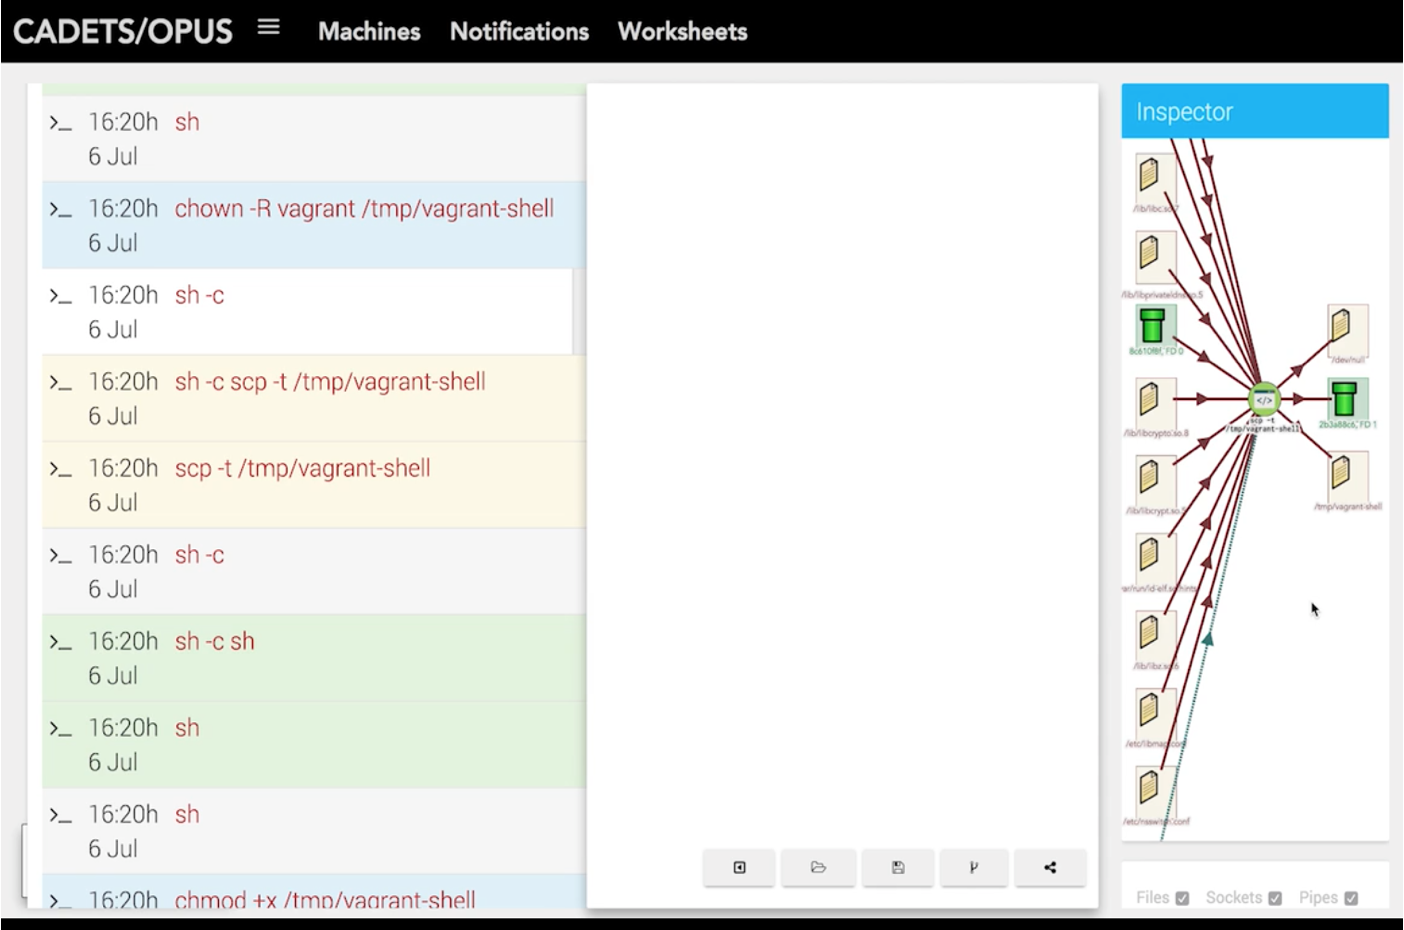
\includegraphics[width=0.7\textwidth]{graphics/CADETS}
		\label{Figure 1.1}
		\caption{\bf Snapshot of CADETS UI}
	\end{figure}
	
	\subsection{Aims of the project}
	In general, the number of nodes that are of interest to the analyst is significantly lower than the number of nodes that are not. Therefore, the aim of this project is to asses the suitability of different machine learning algorithms that would significantly improve the analyst's experience by reducing the number of nodes he would have to manually inspect. 
	
	\section{Overview of the architecture}\label{1.2}
	The main component of the project is a supervised learning algorithm that classifies nodes from the graph as being of interest or not. The model is built using a labelled training set constructed based on a set of predefined ground-truths.
	\\ \\
	The communications between the CADETS user interface and the machine learning model is facilitated by a REST API(as shown in Figure \ref{Figure 1.2}). For performance purposes, it also uses a local cache of previous classifications. 
	\\ \\ 
	When it receives a request from the client, the server would first check the local cache. If it can find the classification result for that node, then it just returns the cached value to the client.
	\begin{figure}[H]
		\centering
		\includegraphics[width=0.8\textwidth]{graphics/overview}
		\label{Figure 1.2}
		\caption{\bf Overview of the project's architecture}
	\end{figure}
	
	If the result is not in the cache or if the cached value expired, it runs the machine learning model in order to classify that specific node. Once the classification is done, the result is stored in the local cache and returned to the client. 
	
	\section{Related work}
	Cyber security has always been a major concern in computer science, both in industry and in research. With the recent interest shown in artificial intelligence and machine learning, there has been an increasing number of tools that use related methodologies to identify malicious behaviour. This section will address some of these tools. 
	
	\subsection{Clearcut}
	Clearcut\footnotemark[1] is an open source tool that uses Machine Learning techniques for incident detection. It takes HTTP proxy logs as input and filters them for manual review, in order to aid the analyst in reviewing them. 
	\\ \\ 
	The algorithm used in this case is Random Forrest Classification, which essentially means having multiple decision trees in training. The returned class is corresponding to the mode of the classes returned by the decision trees running separately. 
	\\ \\
	Compared to Clearcut, the project described in this dissertation takes the inputs as a graph, thus taking into consideration the logs as well as the relationships between them. 
	\footnotetext[1]{\textbf{\url{https://github.com/DavidJBianco/Clearcut}}}
	
	\subsection{Polonium}
	Polonium is a scalable and effective technology that uses graph mining for malware detection. The tool uses a bipartite graph whose nodes describe machines and files as its training data. It uses the Belief Propagation algorithm, which, at a high level, infers the label of a node from some prior knowledge about the node and from the node's neighbours. This is done through iterative message passing between all pairs of nodes $(u, v)$ in the graph. 
	\\ \\
	Although the problem statement is similar to that my project tries to address, the algorithm used here is not applicable in my case, because it requires a very large dataset (Polonium uses a graph with $\approx 1$ billion nodes). It also requires a pre-computed \textit{machine reputation} score that in this case is calculated using a proprietary formula of Symantec\footnotemark[2], the company that produced the tool. 
	\\ \\
	Polonium works at a much higher level in terms of events compared to what my project attempts. Namely, it uses a significantly coarser grained graphs, with a lower diversity of objects: it only takes into consideration files and machines, while the dataset I used also includes processes, sockets and pipes. 

	\footnotetext[2]{\textbf{\url{https://www.symantec.com/}}}
	
	\section{Licence} 
	The code is publicly available as an open-source project on GitHub\footnotemark[3], under an APACHE 2.0 licence\footnotemark[4]. 
	
	
	\footnotetext[3]{\textbf{\url{https://github.com/a96tudor/Part2Project}}}
	\footnotetext[4]{\textbf{\url{https://www.apache.org/licenses/LICENSE-2.0}}}
\end{document}